%%
%%
%%      SECTION: MAIN BEAM 
%%
%%__________________________________________________________________
\section{Main beam {\color{blue} Laurence $\&$ Jean-Fran\c cois}}
\label{se:MB}


We define NIKA2 main beam as the principal Gaussian (of the smaller FWHM)
that encloses most of the measured source flux. The best-fitting value
of the principal-power smaller-FWHM Gaussian function of the
three-Gaussian model, as discussed in Sect.~\ref{se:fullbeam_prof},
provides us with a first estimate of the main beam, which is given in
Table~\ref{tab:fwhm}. However,
this estimate could be biased toward the lower FWHM values due to
degeneracies between the three-Gaussian model parameters. To ensure
obtaining robust main beam FWHM estimates, we devise
{\color{magenta} two} alternative dedicated
methods, which both resort to masking the side lobes: {\color{magenta}
  \i) Gaussian fits of the beam profile to benefit from the
  signal-over-noise increase after azimuthally averaging the signal,}
ii)
Elliptical Gaussian fits of the beam map for a better 2D modeling.
Cross-checking the outputs from these complementary methods is an
important robustess test of our results.

We also consider different data sets acquired during \emph{N2R8}, \emph{N2R9}
and \emph{N2R10}: i) a series of $8' \times 5'$ OTF
scans of primary and secondary calibrators, ii) beam-map scans of
Planets.
{\color{magenta} LP: to repeat this analysis using N2R9, N2R12 and N2R14}

Table~\ref{tab:fwhm} gathers the main beam FWHM results obtained using the three
discussed methods and two datasets.  


\subsection{Sidelobe-masked Profile-based analysis}

{\bf add a description here [Jean-Francois's method]}

\subsection{Sidelobe-masked Map-based analysis}

\paragraph{Method description}

NIKA2 main beam two-dimensionnal distribution is modeled using an elliptical Gaussian. We characterize NIKA2 resolution by giving the \emph{FWHM}, defined as
\begin{equation}
  FWHM = 2 \sqrt{2\ln {2}} \sqrt{\sigma_x\sigma_y},
\end{equation}
where $\sigma_x$ and $\sigma_y$ are the Gaussian standard deviation along minor- and major-axis. To avoid the side lobes contamination, we use masked versions of the beam map, in which an annulus of inner radius $r_{\rm{in}}$ and outter radius $r_{\rm{out}}$ is cut out. Whereas $r_{\rm{out}}$ is conservately set to be $100 arcsec$, $r_{\rm{in}}$ is let free to vary around a central value about $8'$ for A1 and A3 and about $12'$ for A2 to provide the best 2D Gaussian fit.  

\paragraph{Estimates using $8' \times 5'$ OTF scans}

\begin{figure}[ht!]
\begin{center}
  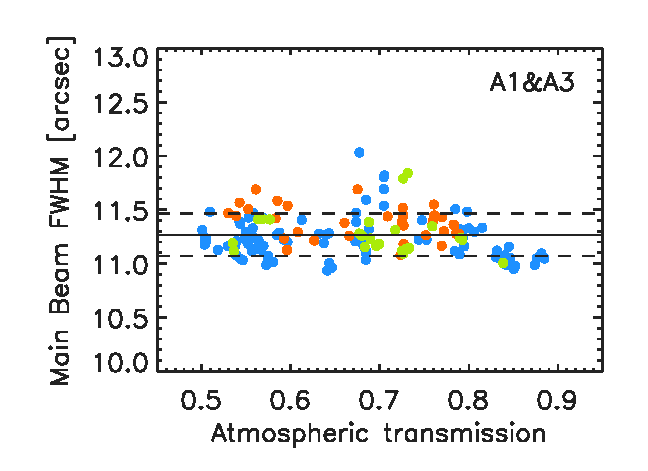
\includegraphics[clip, width=0.45\textwidth]{Figures/Beams/plot_FWHM_vs_atmtrans_mb_radius_binning2_1mm.pdf}
  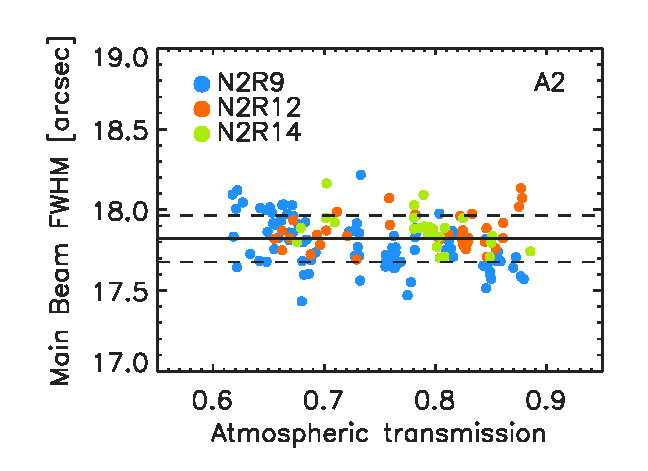
\includegraphics[clip, width=0.45\textwidth]{Figures/Beams/plot_FWHM_vs_atmtrans_mb_radius_binning2_a2.pdf}
  \caption[Main Beam FWHM]{Main beam FWHM estimates for the $1\,\rm{mm}$ (left) and $2\,\rm{mm}$ (right) channels are shown as a function of the atmospheric transmission using bright source scans acquired during N2R9, N2R12 and N2R14. }
\label{fig:fwhm_map_atmtrans}
\end{center}
\end{figure}

We select \emph{N2R9} and \emph{N2R10} $8' \times 5'$ OTF scans of
bright point sources, including primary and secondary
calibrators. Namely, we consider scans of Uranus, Neptune, 3C273,
3C84, 0316+413, Vesta and MWC349, whereas we avoid CRL2688 and
NGC7027, which are slightly extended. Conservative data selection
criteria with respect to observing conditions are applied: average
elevations $\rm{el} \ge 20 \rm{deg}$, zenith opacities as estimated by
NIKA2 in the 1mm band $\tau_{1\rm{mm}} \le 0.4$, reasonable lateral
focus settings $x, y \le 0.5$mm. After selection cuts, our data set
includes 130 OTF scans acquired during \emph{N2R9}, which consists of
a representative sub-sample of a typical NIKA2 observation campaign,
as well as {\bf XXX [TBC]} scans of \emph{N2R10}. 

Figure~\ref{fig:fwhm_map} shows FWHM distributions obtained using
the elliptical Gaussian fit method from the selected set of $8' \times 5'$ OTF scans.
We checked a posteriori that $r_{\rm{in}}$ distributes as $7 \pm 1.5$ arcsec at 1mm and $13 \pm 4$ arcsec at 2mm, in agreement with settings defined in the profile-based analysis.


\begin{figure}[ht!]
\begin{center}
  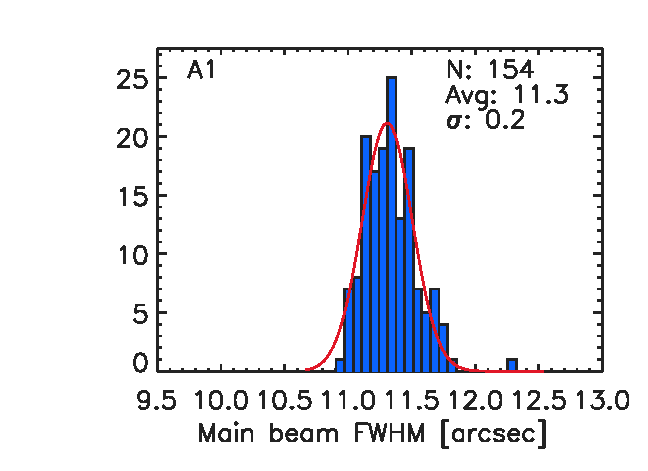
\includegraphics[clip, width=0.42\textwidth]{Figures/Beams/plot_histo_FWHM_mb_radius_binning2_a1.pdf}
  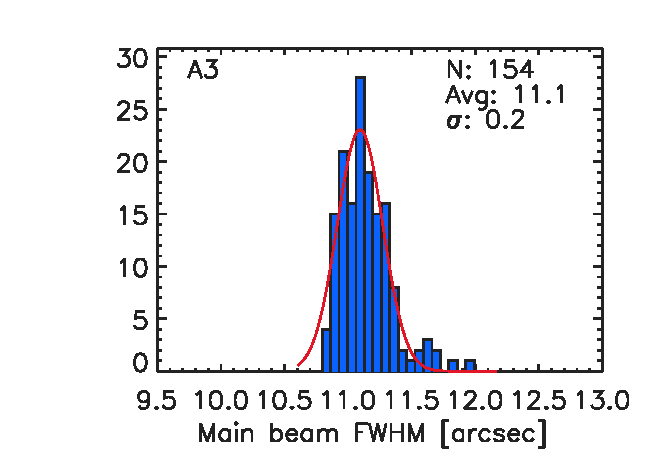
\includegraphics[clip, width=0.42\textwidth]{Figures/Beams/plot_histo_FWHM_mb_radius_binning2_a3.pdf}
  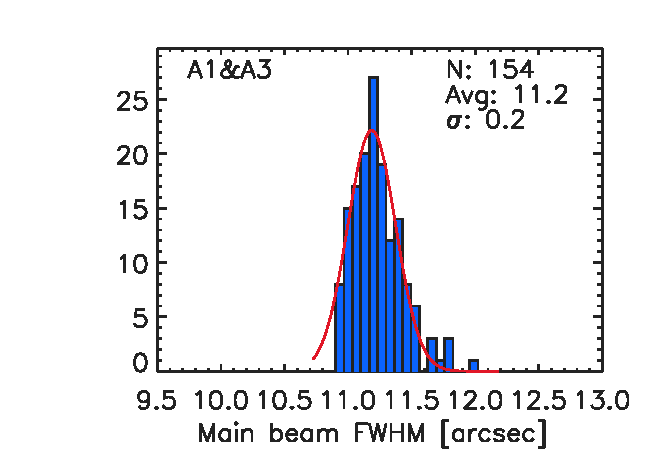
\includegraphics[clip, width=0.42\textwidth]{Figures/Beams/plot_histo_FWHM_mb_radius_binning2_1mm.pdf}
  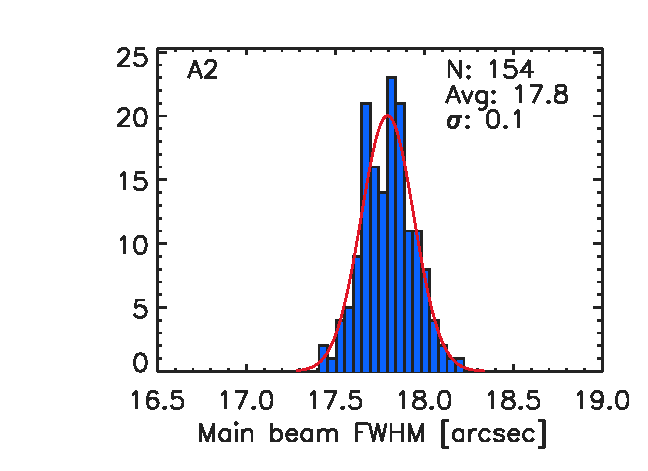
\includegraphics[clip, width=0.42\textwidth]{Figures/Beams/plot_histo_FWHM_mb_radius_binning2_a2.pdf}
  \caption[Main Beam FWHM distributions]{Distribution of the FWHM estimates for Array 1, 3, the comination of Array $1\&3$ and Array 2, including bright source scans from the three campaigns.}
\label{fig:fwhm_map}
\end{center}
\end{figure}

\paragraph{Estimates using beam-map scans}

We use masked version of the beam maps, which are selected as
described in Sect.~\ref{se:beammap_set}. 
Sidelobe masks are defined by a fixed $r_{\rm{out}}$ of $100 arcsec$
and a $r_{\rm{in}}$ that freely varies from $8'$ to $9'$ for the
$260~\rm{GHz}$-arrays, and from $10'$ to $14'$ for the $150~\rm{GHz}$
array. We checked, hovewer, that we obtain consistent results but
larger dispersion when using annulus masks of fixed $r_{\rm{in}}$ of
$8.5'$ and $12'$ at $260$ and $150~\rm{GHz}$ respectively. The median
main beam FWHM and the rms error estimate, which have been obtained
from the nine beam-maps, are given in Table~\ref{tab:fwhm}.

\begin{table}[h]
  \caption[]{FWHM of the NIKA2 main beam in arcsec.}
  \centering
  \begin{threeparttable}
  \begin{tabular}{|l|c|c|c|c|c|}
    \hline
    
       &    &  \multicolumn{4}{|c|}{Array or array combination} \\
    \cline{3-6}
    Method & Dataset        &   A1 &  A3 & A1 $\&$ A3 &  A2  \\
    \hline
    \hline
    Three-Gaussian model G1\tnote{a} &  beam-map &  $10.8 \pm 0.2$  &  $10.8 \pm 0.2$  &  $10.8 \pm 0.3$  &  $17.2 \pm 0.05$  \\
    Sidelobe-masked profile-based    &  TBD      &    &    &    &   \\
    Sidelobe-masked map-based        &  OTF       & $11.0 \pm 0.3$  &  $10.9 \pm 0.2$  &  $11.0 \pm 0.2$  &  $17.8 \pm 0.2$ \\ 
                                     &  beam-map  & $11.3 \pm 0.2$  & $11.2 \pm 0.2$   &  $11.2 \pm 0.2$  &  $17.7 \pm 0.05$ \\ 
    \hline
  \end{tabular}
  \begin{tablenotes}
  \item[(a)] Median FWHM of the first (lowest-FWHM) Gaussian function
    within the Three-Gaussian model fitted from the beam-map scan selection 
  \end{tablenotes}
  \end{threeparttable}
  \label{tab:fwhm}
\end{table}

\subsection{FWHM distribution across the FoV}

% COPY FROM THE 'INSTRUMENT' PAPER
\begin{figure}[ht!]
  \centering
  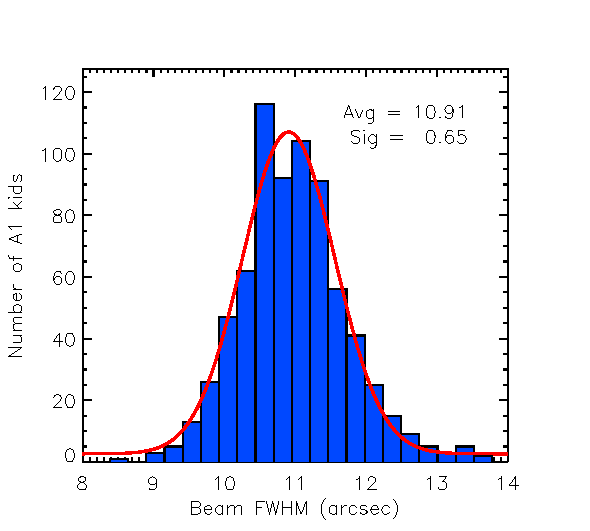
\includegraphics[clip=true,width=0.45\textwidth]{../../../Paper_NIKA2_Technical/plot_histo_A1_fwhm_20170424s123.pdf}
  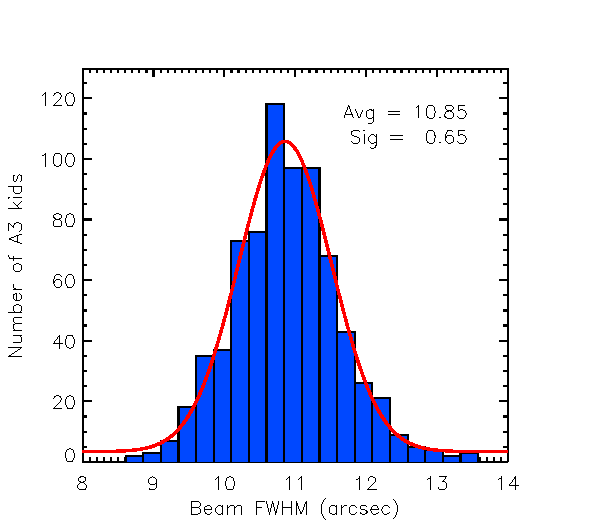
\includegraphics[clip=true,width=0.45\textwidth]{../../../Paper_NIKA2_Technical/plot_histo_A3_fwhm_20170424s123.pdf}
  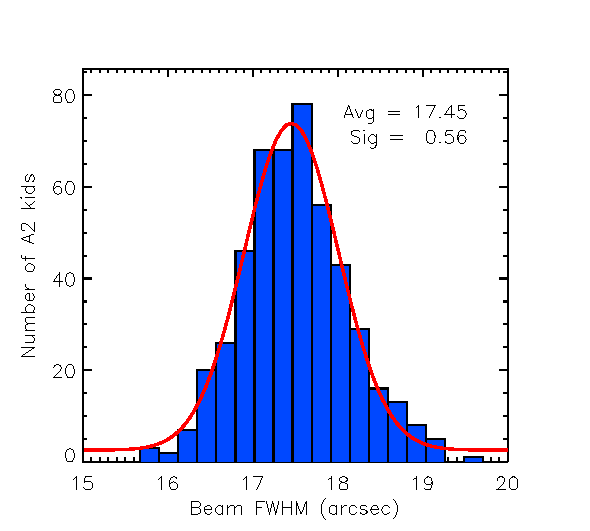
\includegraphics[clip=true,width=0.45\textwidth]{../../../Paper_NIKA2_Technical/plot_histo_A2_fwhm_20170424s123.pdf}
  
\caption[Main beam FWHM distribution across the array]{Main beam FWHM distribution of all valid KID detectors of arrays A1, A3, and A2. The main beam FWHM is the geometrical combination of the two-orthogonal FWHM estimates obtained from an elliptical Gaussian fit on side-lobe masked individual maps per KID (see text). The red curves show a Gaussian fit to the histogram data.}
  \label{fig:focalplane_histo}
\end{figure}

Figure \ref{fig:focalplane_histo} shows the distribution of the
main beam FWHMs of the arrays A1, A3 and A2 using a beammap
scan of Neptune acquired during the April 2017 commissioning
campaign and for average weather conditions (scan ID: 20170424s123). We also
show in red the best Gaussian fit to histogram data. We find an
average main beam FWHM of $10.9''$ at 260 GHz and $17.5''$ at
150 GHz in agreement with the main beam estimates gathered in
Table~\ref{tab:fwhm}.
The observed dispersion of about $0.6''$ is expected from the optics desing and its associated
field distortions across the 6.5 arc-minutes FoV, as discussed in
Sect.~\ref{se:grid_distortion}. This quantifies the impact of the
non-constant focus across the FoV, which is characterised in
Sect.~\ref{sec:focus-surf}, on the individual detector main beams.  





